\documentclass[12pt, oneside]{article}

\usepackage{./texmf/preamble}
% \usepackage{subfiles}

\graphicspath{{./assets/}}
\addglobalbib{refs.bib}

\pagestyle{normal}
\onehalfspacing

\providecommand{\wordcount}{222}

% =================================================================
% Content
% =================================================================

\begin{document} % BEGIN
\pagestyle{normal}

\begin{titlepage}
    \large

    \begin{center}

        \vspace*{2cm}

        {\bfseries
            IB Math Analysis and Approaches (HL) \\
            Extended Essay\\
            May 2024 Session}\\

        \vspace*{\fill}

        \rule{\linewidth}{1.5pt} \\ [0.5cm]
        {\LARGE \bfseries Understanding and Applying the Fundamental Principles of Camera Calibration}
        \rule{\linewidth}{0.5pt} \\

        \vspace*{\fill}

        \textbf{Research Question:} What mathematical techniques can be employed to create precise camera models for accurately converting 2D image data into 3D point reconstructions, and what are their practical applications in real-world scenarios? \\ [1cm]

        \textbf{Word Count:} \wordcount \space words

        \vspace*{2cm}

    \end{center}

\end{titlepage}

% =================================================================
\pagenumbering{roman}
\thispagestyle{empty}
\tableofcontents
% =================================================================
\clearpage
\pagenumbering{arabic}
\setcounter{page}{1}

\section{Introduction}

Camera calibration is an important process in computer vision and computer graphics which involves determining the parameters of a camera. The knowledge of these parameters are essential, because it allows us to create a mathematical model which accurately describes the camera. Without a well-calibrated camera, images captured may suffer from inaccuracies and distortion, making calibration an indispensable step in a wide array of applications.

While manufacturers of cameras often report parameters of cameras, such as the nominal focal length and pixel sizes of their camera sensor, these figures are typically approximations which can vary from camera to camera, particularly in consumer-grade cameras. As such, the use of these estimates by manufacturers are unsuitable to be used in applications requiring high accuracy. Combined with the potential for manufacturing defects as well as lens distortion effects further necessitates the need for a reliable method for determining the parameters of a camera. Camera calibration emerges as the answer to these problems, allowing us to create very accurate estimates for the parameters of a camera. 

Photogrammetry, as a comprehensive science, concerns itself with obtaining precise measurements of 3-dimensional physical objects from photographic images. 

It was first employed by Prussian architect Albrecht Meydenbauer in the 1860s, who used photogrammetric techniques to create some of the most detailed topographic plans and elevations drawings \autocite{ices2017}. 
Camera calibration borrows techniques from photogrammetry 

Today, photogrammetric techniques are used in a multitude of applications spanning diverse fields, including computer vision, topographical mapping, medical imaging, and forensic analysis.

Importance of reserach question

In order to accurately determine the position of 3D points based on data from multiple 2D images, we must have knowledge of the parameters of the camera.

This process of calculating




The task of generating an accurate 3D model from various 2D images is a multi-step process, and consists of:




and they mainly fall into two main categories. The first method is based on the cross-referencing of keypoints between the images. Computer algorithms such as SIFT (Scale Invariant Feature Transform) and SURF (Speeded-Up Robust Features)









\section{Literature Review}

There exists many camera calibration methods, however the most common and

Zhang's method and Tsai's method. 

\section{Approach} 

\subsection{Camera Model} \label{sec:camera_model}

A camera model is a projection model that approximates the function of a camera by describing a mathematical relationship between points in 3D space and its projection onto the sensor grid of the camera. In order to accurately model a camera, we must first understand the general workings of a camera.

Modern lens cameras are highly sophisticated, built with an array of complex mechanisms and a wide range of features. The complexity of cameras can be better understood by breaking down their components down into three main elements critical to image projection: the lens, the aperture, and the sensor grid (CCD). 

\begin{figure}[H]
    \centering
    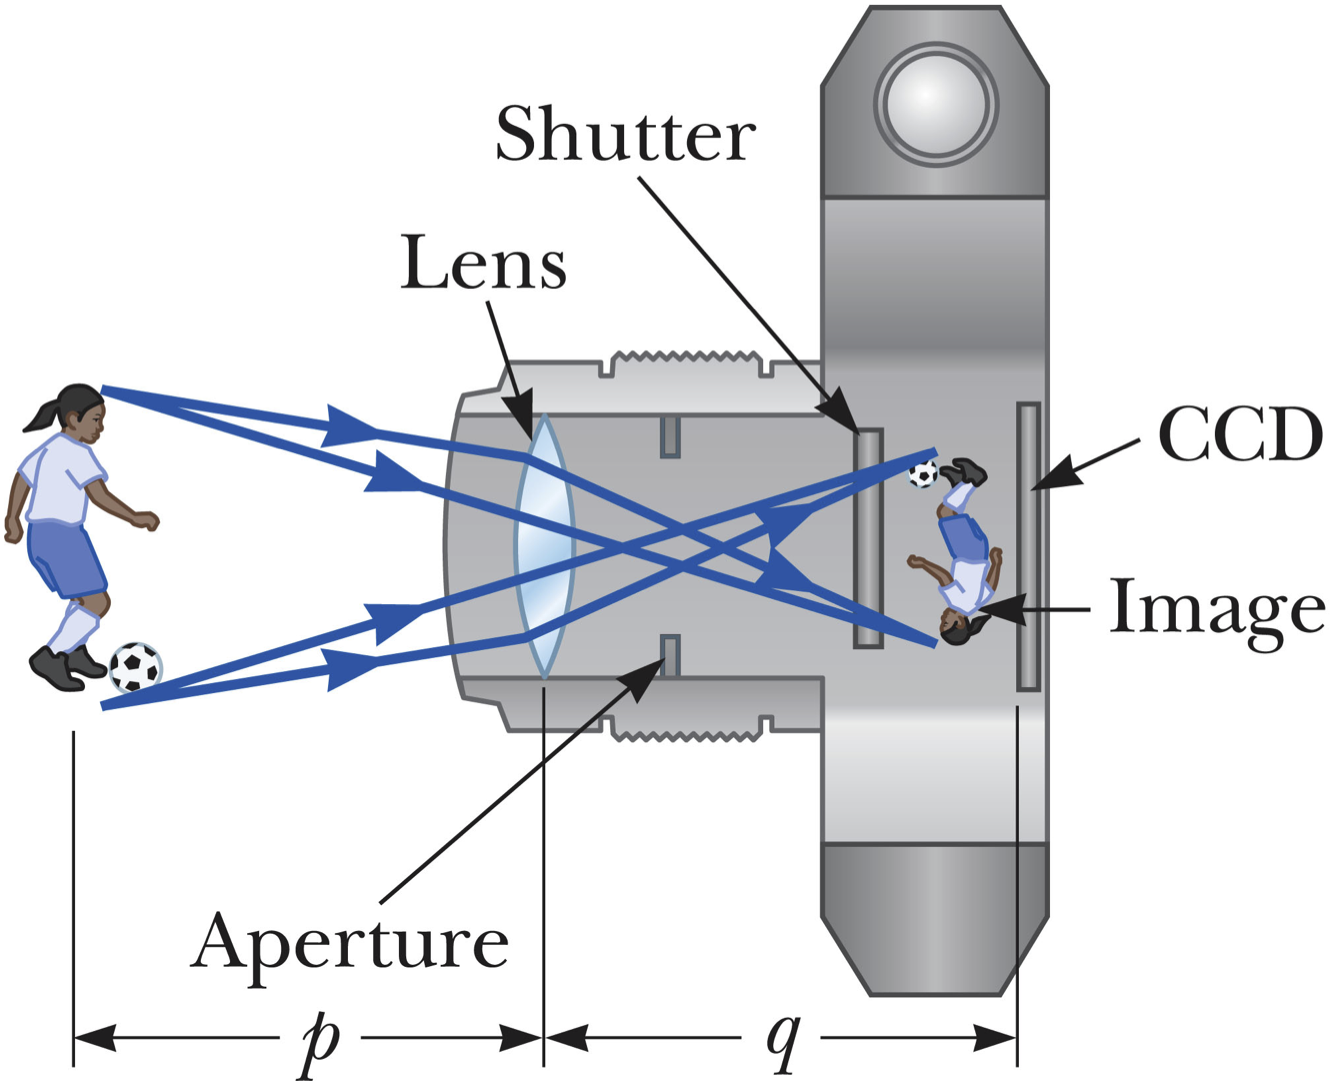
\includegraphics[width=0.5\textwidth]{images/lens_camera}
    \caption{Lens camera. Adapted from \cite{coltonPhysics1232012}} \label{fig:lens_camera}
\end{figure}

The lenses 


However, we can simplify the model of the lens camera by collapsing the mechanisms of the camera into 3 main functional components that are important to the image projection: the lens, the aperture, and the sensor grid (CCD). This simplified model is visualized in Figure \ref{fig:lens_camera}. The lens focuses incoming light rays towards the aperture, before they project inverted onto the sensor grid. However, even this simplified model of a lens camera is too complex to model, as there is no simple mathematical equation which accurately describes the behavior of a lens. As such, we can further simplify our camera model by building upon the pinhole camera model, which is one of the simplest and most commonly used camera models in camera calibration.



A pinhole camera is a simple camera without a lens. Instead, it relies on the use of a tiny hole as the aperture of the camera, and light rays pass through the hole, projecting an inverted image onto the

\begin{figure}[H]
    \centering
    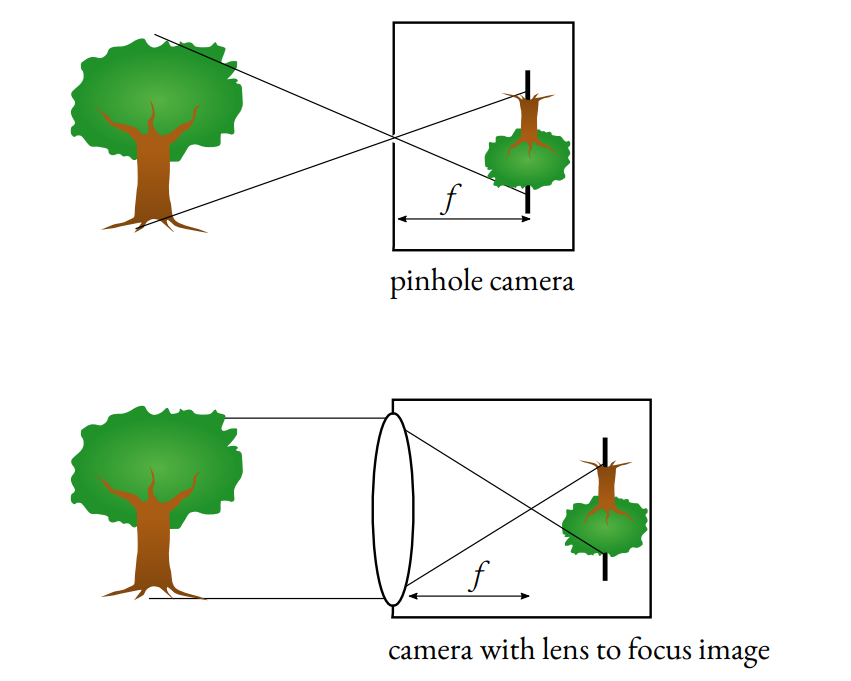
\includegraphics[width=0.7\textwidth]{images/pinhole_vs_lens}
    \caption{Difference between a pinhole camera and a lens camera. Adapted from \cite{leCameraModel2018}}
\end{figure}



There are a few assumptions which are made by the pinhole camera model:

Extremely simple model for imaging geometry
Doesn't strictly apply
Mathematically convenient acceptable approximation.
\begin{itemize}
    \item T
\end{itemize}

The pinhole camera model does not accurately describe the true workings of a camera, as some of the  effects that the model fails to account for can be compensated the errors which results from these assumptions are sufficiently small to be neglected if a high quality camera is used. Additionally,

\begin{figure}[H]
    \centering
    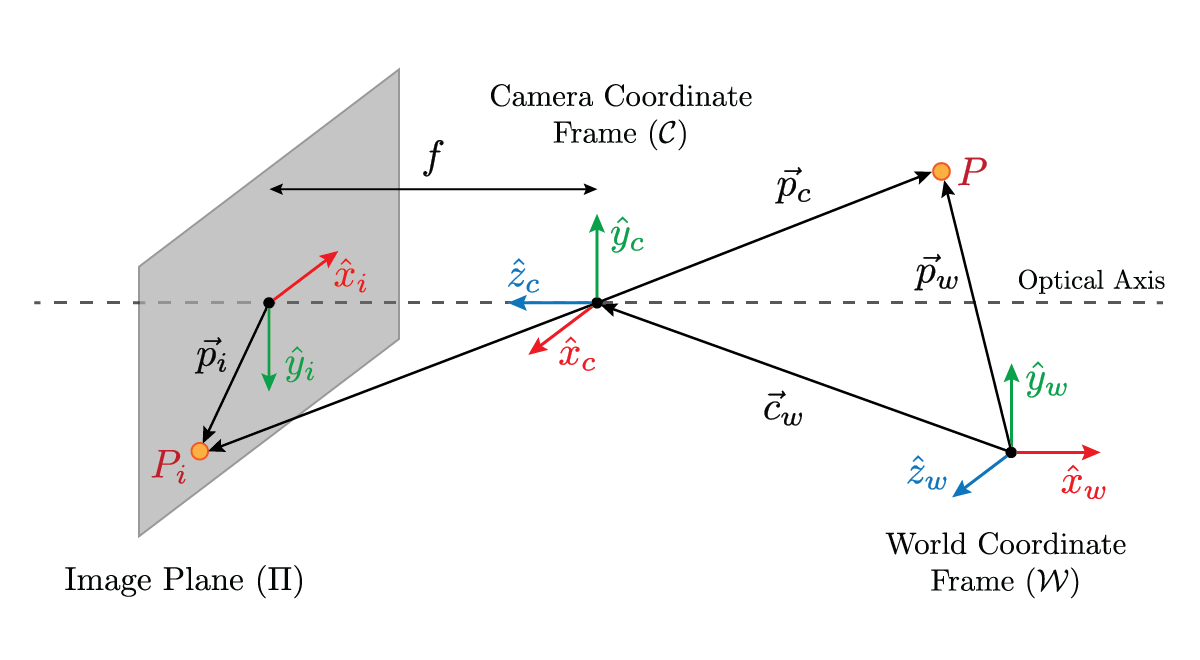
\includegraphics[width=0.9\textwidth]{figures/imaging_model}
    \caption{Pinhole camera model.}
\end{figure}

\subsubsection{Geometry}


For our camera model, we will establish 3 frames of


\begin{figure}[H]
    \centering
    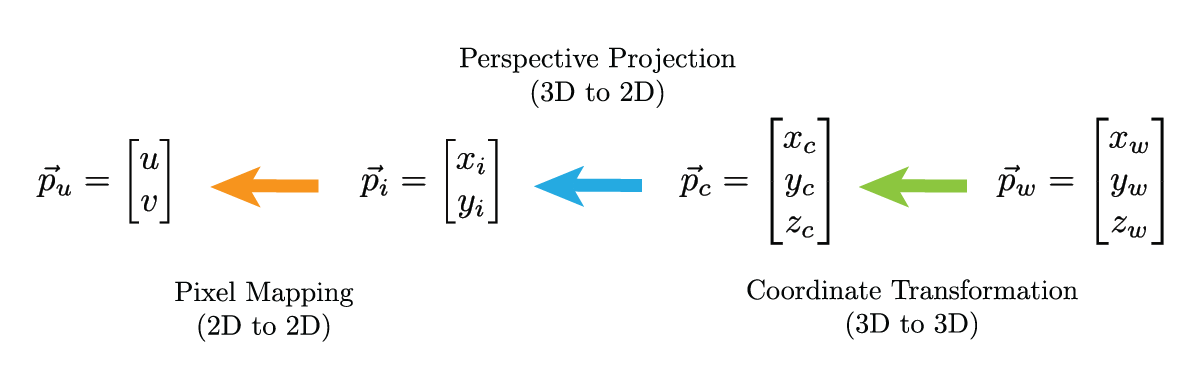
\includegraphics[width=0.9\textwidth]{figures/coord_conversions}
    \caption{Coordinate remappings.}
\end{figure}





There are countless different approaches one could take to calibrate a camera, 



however they all build upon techniques first described in multiple highly influential papers, most notably Tsai's ``A Versatile Camera Calibration Technique for High-Accuracy 3D Machine Vision Metrology Using Off-the-shelf TV Cameras and Lenses'' and Zhang's ``A Flexible New Technique for Camera Calibration''. 

\subsection{Calibration Object}

Calibration techniques can be roughly separated into 3 categories, based on the dimension of the calibration object used \footcite{zhangCameraCalibration2007}:


\section{Intrinsic Parameters}

\begin{figure}[h!]
    \centering
    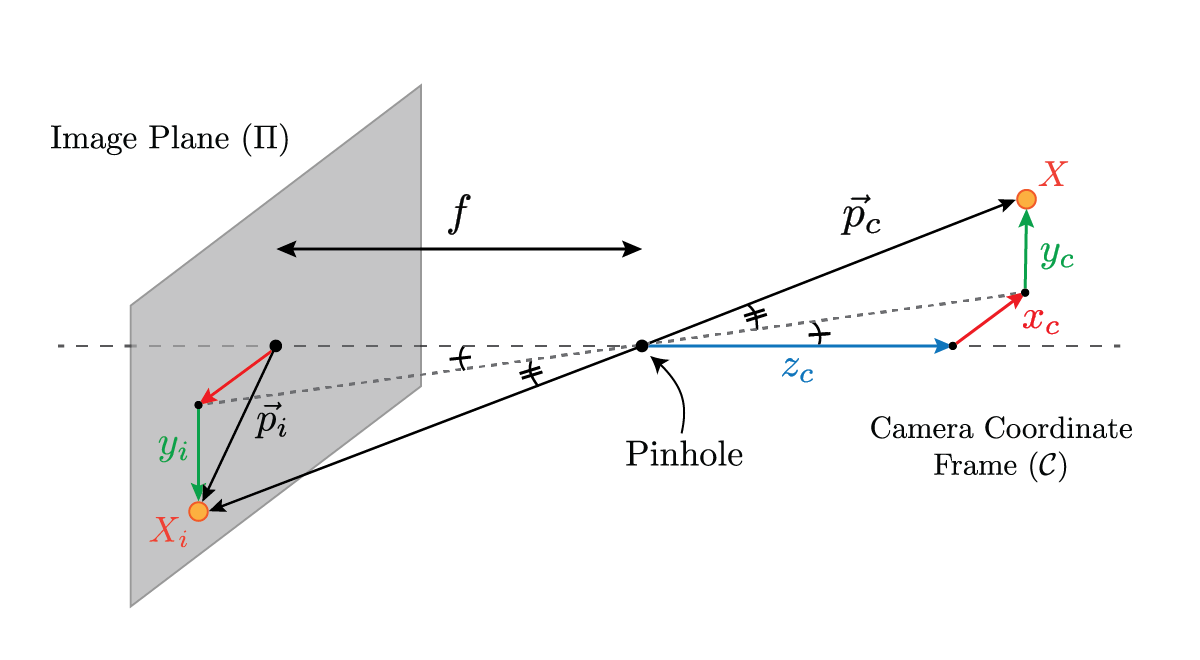
\includegraphics[width=0.9\textwidth]{figures/perspective_projection}
    \caption{Perspective projection.}
\end{figure}

\begin{equation}
    \vec{p}_i = M_{int} \vec{p}_c
\end{equation}

\begin{figure}[h!]
    \centering
    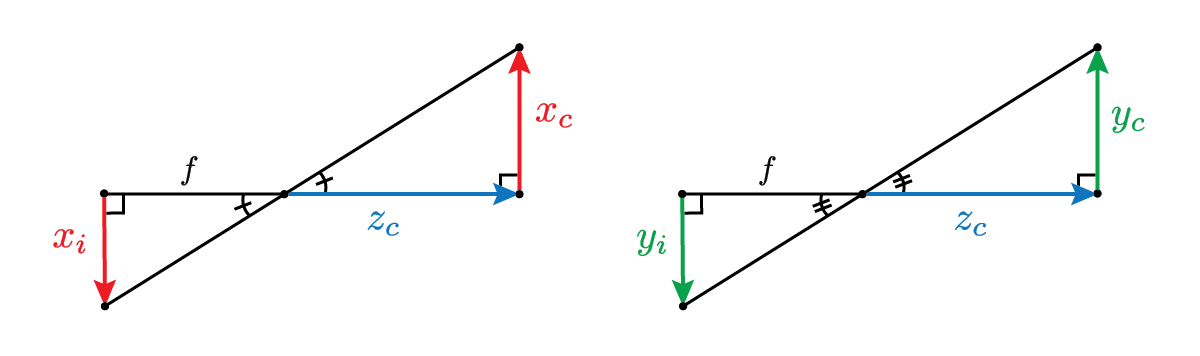
\includegraphics[width=0.9\textwidth]{figures/similar_triangles}
    \caption{Similar triangles.}
\end{figure}

\begin{gather}
    \frac{x_i}{f} = \frac{x_c}{z_c} \Rightarrow x_i = f \frac{x_c}{z_c} \\
    \frac{y_i}{f} = \frac{y_c}{z_c} \Rightarrow y_i = f \frac{y_c}{z_c}
\end{gather}


Let $m_x$ and $m_y$ represent the pixel density of the image sensor in the $x$ and $y$ axes of the image sensor plane respectively.


\begin{gather}
    u = m_x x_i + c_x \\
    v = m_y y_i + c_y
\end{gather}

\begin{gather}
    u = m_x f \frac{x_c}{z_c} + c_x \\
    v = m_y f \frac{y_c}{z_c} + c_y
\end{gather}

\begin{gather}
    u = f_x \frac{x_c}{z_c} + c_x \\
    v = f_y \frac{y_c}{z_c} + c_y
\end{gather}

\begin{equation}
    \begin{bmatrix}
        u \\ v \\ 1
    \end{bmatrix}
    \cong
    \begin{bmatrix}
        z_c u \\ z_c v \\ z_c
    \end{bmatrix}
    =
    \begin{bmatrix}
        f_x x_c + z_c c_x \\ f_y y_c + z_c c_y \\ z_c
    \end{bmatrix}
    =
    \underbrace{
        \begin{bmatrix}
            f_x & 0   & c_x & 0 \\
            0   & f_y & c_y & 0 \\
            0   & 0   & 1   & 0
        \end{bmatrix}
    }_{=M_{int}}
    \begin{bmatrix}
        x_c \\ y_c \\ z_c \\ 1
    \end{bmatrix}
\end{equation}

\section{Coordinate Transformation} \label{sec:extrinsics}

First, we 

Now, we would like to find the extrinsic matrix, $M_{ext}$, which relates the positional vector $\vec{p}_w$ of point $P$ in the world coordinate frame, to its positional vector $\vec{p}_c$ in the camera coordinate frame. Similar to what we did in section \ref{sec:intrinsics}, we can express this in homogenous coordinates as follows:
\begin{equation} \label{eq:pc}
    \widetilde{p}_c =  M_{ext}\,\widetilde{p}_w
\end{equation}

\begin{figure}[H]
    \centering
    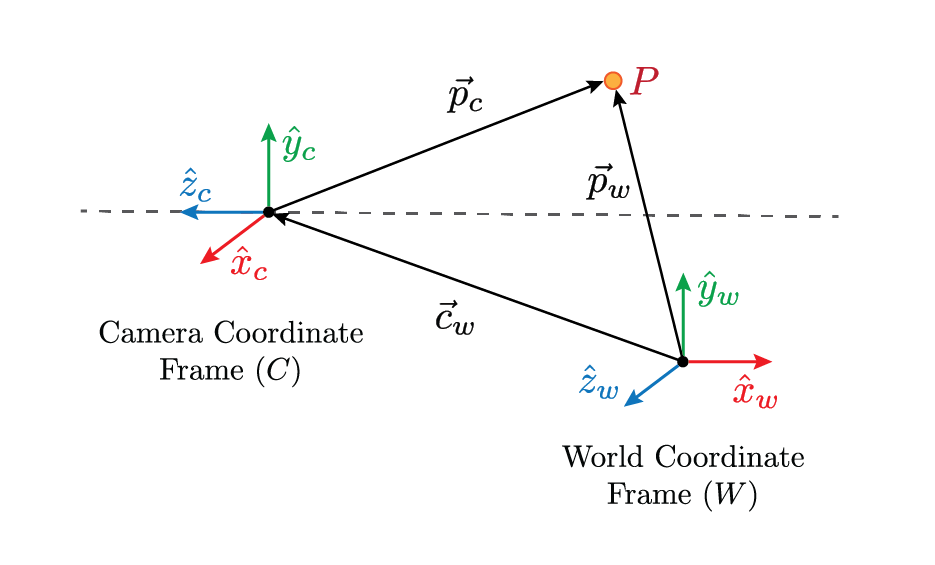
\includegraphics[width=0.9\textwidth]{figures/coord_transform}
    \caption{Coordinate transformation from the world coordinate frame to the camera frame.}
\end{figure}

\subsection{Extrinsic Matrix}

For the extrinsic parameters of the camera, we have the position $\vec{c}_w$ of the camera in world coordinates and orientation $R$ of the camera. The orientation, $R$, is a 3x3 rotational matrix: 

\begin{equation}
    R = 
    \begin{bmatrix}
        r_{11} & r_{12} & r_{13} \\
        r_{21} & r_{22} & r_{23} \\
        r_{31} & r_{32} & r_{33}
    \end{bmatrix}
\end{equation}

\noindent where:
\begin{itemize}
    \item Row 1: Direction of $\hat{x}_c$ in world coordinate frame.
    \item Row 2: Direction of $\hat{y}_c$ in world coordinate frame.
    \item Row 3: Direction of $\hat{z}_c$ in world coordinate frame.
\end{itemize}

\noindent 

\begin{subequations}
    \begin{align}
        \vec{p}_c & = R(\vec{p}_w-\vec{c}_w) \\
                  & = R\vec{p}_w -R\vec{c}_w  
    \end{align}
\end{subequations}



\begin{gather}
    \vec{p}_c = R\vec{p}_w + \vec{t} \\
    \begin{bmatrix}
        x_c \\ y_c \\ z_c
    \end{bmatrix}
    =
    \underbrace{
        \begin{bmatrix}
            r_{11} & r_{12} & r_{13} \\
            r_{21} & r_{22} & r_{23} \\
            r_{31} & r_{32} & r_{33}
        \end{bmatrix}
    }_{\mathlarger{R}}
    \begin{bmatrix}
        x_w \\ y_w \\ z_w
    \end{bmatrix}
    +
    \underbrace{  
        \begin{bmatrix}
            t_x \\ t_y \\ t_z
        \end{bmatrix}
    }_{\mathlarger{\vec{t}}}
\end{gather}


\begin{equation}
    \begin{bmatrix}
        x_c \\ y_c \\ z_c \\ 1
    \end{bmatrix}
    =
    \underbrace{
        \begin{bmatrix}
            r_{11} & r_{12} & r_{13} & t_x \\
            r_{21} & r_{22} & r_{23} & t_y \\
            r_{31} & r_{32} & r_{33} & t_z \\
            0      & 0      & 0      & 1
        \end{bmatrix}
    }_{\mathlarger{M_{ext}}}
    \begin{bmatrix}
        x_w \\ y_w \\ z_w \\1
    \end{bmatrix}
\end{equation}

\begin{equation}
    M_{ext} = 
    \begin{bmatrix}
        R_{3 \times 3} & t_{3 \times 1} \\
        0_{1 \times 3} & 1
    \end{bmatrix} 
\end{equation}

\section{Handling Distortion}

When constructing our camera model in section \ref{sec:camera_model}, we made the assumption that the camera we are using can be approximated using a pinhole camera.


Modern cameras rarely have a single lens. Rather, they typically have compound lens




\subsection{Symmetrical Radial Distortion}

Symmetrical lens distortion refers to

It


\begin{figure}[h!]
    \centering
    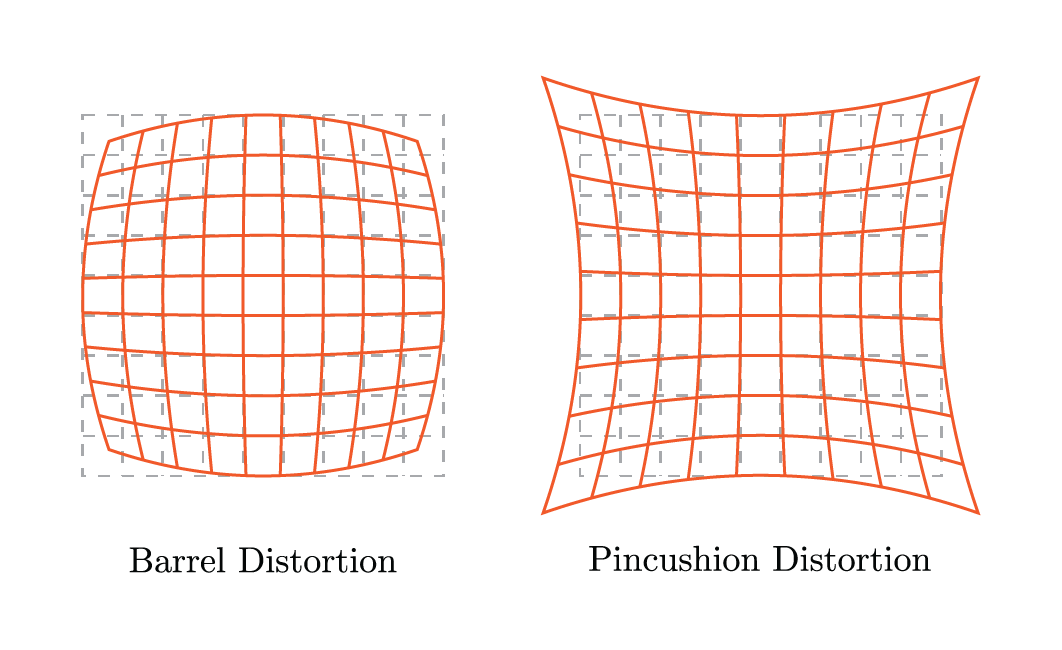
\includegraphics[width=0.9\textwidth]{images/radial_distortion}
    \caption{Types of radial distortion.}
\end{figure}

\subsection{Asymmetrical Radial Distortion}

\subsection{Tangential (Decentering) Distortion}

of axis

\begin{figure}[h!]
    \centering
    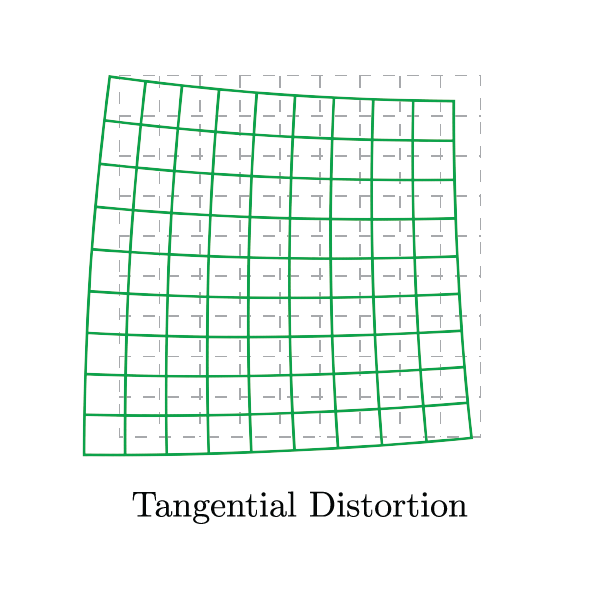
\includegraphics[width=0.45\textwidth]{images/tangential_distortion}
    \caption{Tangential (Decentering) Distortion}
\end{figure}

\begin{figure}[h!]
    \centering
    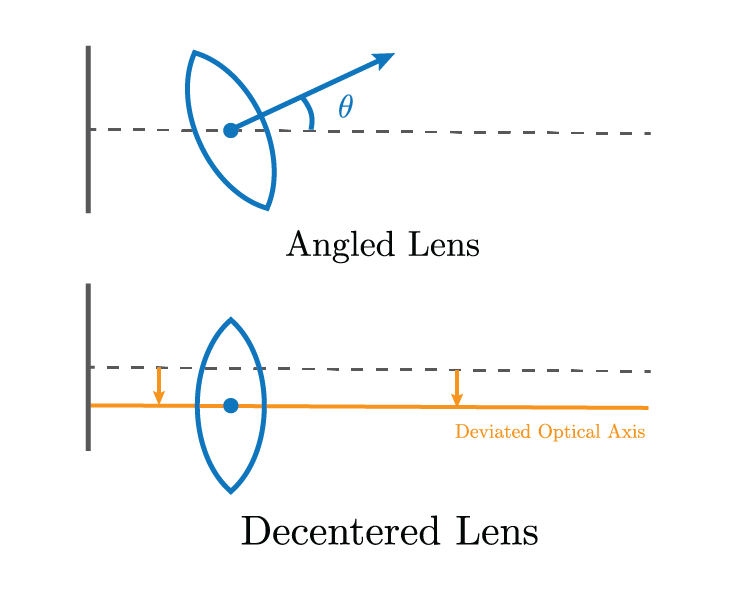
\includegraphics[width=0.5\textwidth]{figures/lens_alignment}
    \caption{Reasons why tangential distortion can occur}
\end{figure}

\subsection{Brown-Conrady Model}

\section{Putting It Together}
\begin{equation}
    \vec{p}_{i_{(n)}} = \underbrace{M_{int}M_{ext}}_{=P}\vec{p}_{w_{(n)}}
\end{equation}

\begin{equation}
    \begin{bmatrix}
        u_n \\ v_n \\ 1
    \end{bmatrix}
    \cong
    \begin{bmatrix}
        \widetilde{w}_n u_n \\ \widetilde{w}_n v_n \\ \widetilde{w}_n
    \end{bmatrix}
    =
    \begin{bmatrix}
        \widetilde{u}_n \\ \widetilde{v}_n \\ \widetilde{w}_n
    \end{bmatrix}
    =
    \underbrace{
        \begin{bmatrix}
            p_{11} & p_{12} & p_{13} & p_{14} \\
            p_{21} & p_{22} & p_{23} & p_{24} \\
            p_{31} & p_{32} & p_{33} & p_{34}
        \end{bmatrix}
    }_{=P}
    \begin{bmatrix}
        x_w^{(n)} \\ y_w^{(n)} \\ z_w^{(n)} \\ 1
    \end{bmatrix}
\end{equation}

\begin{align}
        \widetilde{u}_n = p_{11}x_w^{(n)} + p_{12}y_w^{(n)} + p_{13}z_w^{(n)} + p_{14} \\
        \widetilde{v}_n = p_{21}x_w^{(n)} + p_{22}y_w^{(n)} + p_{23}z_w^{(n)} + p_{24} \\
        \widetilde{w}_n = p_{31}x_w^{(n)} + p_{32}y_w^{(n)} + p_{33}z_w^{(n)} + p_{34}
\end{align}


\begin{align}
    u_n = \frac{\widetilde{u}_n}{\widetilde{w}_n} & = \frac{p_{11}x_w^{(n)} + p_{12}y_w^{(n)} + p_{13}z_w^{(n)} + p_{14}}{p_{31}x_w^{(n)} + p_{32}y_w^{(n)} + p_{33}z_w^{(n)} + p_{34}} \\
    v_n = \frac{\widetilde{v}_n}{\widetilde{w}_n} & = \frac{p_{21}x_w^{(n)} + p_{22}y_w^{(n)} + p_{23}z_w^{(n)} + p_{24}}{p_{31}x_w^{(n)} + p_{32}y_w^{(n)} + p_{33}z_w^{(n)} + p_{34}}
\end{align}

\begin{align}
    u_n(p_{31}x_w^{(n)} + p_{32}y_w^{(n)} + p_{33}z_w^{(n)} + p_{34}) & = p_{11}x_w^{(n)} + p_{12}y_w^{(n)} + p_{13}z_w^{(n)} + p_{14} \\
    v_n(p_{31}x_w^{(n)} + p_{32}y_w^{(n)} + p_{33}z_w^{(n)} + p_{34}) & = p_{21}x_w^{(n)} + p_{22}y_w^{(n)} + p_{23}z_w^{(n)} + p_{24}
\end{align}

\begin{align}
    0 & = p_{11}x_w^{(n)} + p_{12}y_w^{(n)} + p_{13}z_w^{(n)} + p_{14} - p_{31}u_nx_w^{(n)} - p_{32}u_ny_w^{(n)} - p_{33}u_nz_w^{(n)} - p_{34}u_n \\
    0 & = p_{21}x_w^{(n)} + p_{22}y_w^{(n)} + p_{23}z_w^{(n)} + p_{24} - p_{31}v_nx_w^{(n)} - p_{32}v_ny_w^{(n)} - p_{33}v_nz_w^{(n)} - p_{34}v_n
\end{align}

\setcounter{MaxMatrixCols}{20}
\begin{equation} 
    \scalemath{0.9}{
        \begin{bmatrix}
            0 \\ 0 \\ 0 \\ 0 \\ 0 \\ 0 \\ 0 \\ 0 \\ 0 \\ 0 \\ 0 \\ 0
        \end{bmatrix}
        =
        \underbrace{
            \begin{blockarray}{[*{12}c]}
                x_w^{(1)} & y_w^{(1)} & z_w^{(1)} & 1 & 0         & 0         & 0         & 0 & -u_nx_w^{(1)} & -u_ny_w^{(1)} & -u_nz_w^{(1)} & -u_1 \\
                0         & 0         & 0         & 0 & x_w^{(1)} & y_w^{(1)} & z_w^{(1)} & 1 & -v_nx_w^{(1)} & -v_ny_w^{(1)} & -v_nz_w^{(1)} & -v_1 \\
                \BAmulticolumn{6}{c}{\vdots} & \BAmulticolumn{6}{c}{\vdots} \\
                x_w^{(n)} & y_w^{(n)} & z_w^{(n)} & 1 & 0         & 0         & 0         & 0 & -u_nx_w^{(n)} & -u_ny_w^{(n)} & -u_nz_w^{(n)} & -u_n \\
                0         & 0         & 0         & 0 & x_w^{(n)} & y_w^{(n)} & z_w^{(n)} & 1 & -v_nx_w^{(n)} & -v_ny_w^{(n)} & -v_nz_w^{(n)} & -v_n
            \end{blockarray}
        }_{=A}
        \underbrace{
            \begin{bmatrix}
                p_{11} \\ p_{12} \\ p_{13} \\ p_{14} \\ p_{21} \\ p_{22} \\ p_{23} \\ p_{24} \\ p_{31} \\ p_{32} \\ p_{33} \\ p_{34}
            \end{bmatrix}
        }_{=p}
    }
\end{equation}





\section{Applications}


% =================================================================
\section*{Acknowledgements}
\addcontentsline{toc}{section}{Acknowledgements}

I am very grateful to my supervisor Mr. Hoteit for his continual guidance and invaluable pieces of advice during the process of writing this extended essay. I would also like to thank Aditya, for aiding me with the creation of some diagrams used in this essay. 

\printbibliography[heading=bibintoc]{}

\end{document} % END
